% Options for packages loaded elsewhere
\PassOptionsToPackage{unicode}{hyperref}
\PassOptionsToPackage{hyphens}{url}
\PassOptionsToPackage{dvipsnames,svgnames,x11names}{xcolor}
%
\documentclass[
  letterpaper,
  DIV=11,
  numbers=noendperiod]{scrartcl}

\usepackage{amsmath,amssymb}
\usepackage{iftex}
\ifPDFTeX
  \usepackage[T1]{fontenc}
  \usepackage[utf8]{inputenc}
  \usepackage{textcomp} % provide euro and other symbols
\else % if luatex or xetex
  \usepackage{unicode-math}
  \defaultfontfeatures{Scale=MatchLowercase}
  \defaultfontfeatures[\rmfamily]{Ligatures=TeX,Scale=1}
\fi
\usepackage{lmodern}
\ifPDFTeX\else  
    % xetex/luatex font selection
\fi
% Use upquote if available, for straight quotes in verbatim environments
\IfFileExists{upquote.sty}{\usepackage{upquote}}{}
\IfFileExists{microtype.sty}{% use microtype if available
  \usepackage[]{microtype}
  \UseMicrotypeSet[protrusion]{basicmath} % disable protrusion for tt fonts
}{}
\makeatletter
\@ifundefined{KOMAClassName}{% if non-KOMA class
  \IfFileExists{parskip.sty}{%
    \usepackage{parskip}
  }{% else
    \setlength{\parindent}{0pt}
    \setlength{\parskip}{6pt plus 2pt minus 1pt}}
}{% if KOMA class
  \KOMAoptions{parskip=half}}
\makeatother
\usepackage{xcolor}
\setlength{\emergencystretch}{3em} % prevent overfull lines
\setcounter{secnumdepth}{-\maxdimen} % remove section numbering
% Make \paragraph and \subparagraph free-standing
\makeatletter
\ifx\paragraph\undefined\else
  \let\oldparagraph\paragraph
  \renewcommand{\paragraph}{
    \@ifstar
      \xxxParagraphStar
      \xxxParagraphNoStar
  }
  \newcommand{\xxxParagraphStar}[1]{\oldparagraph*{#1}\mbox{}}
  \newcommand{\xxxParagraphNoStar}[1]{\oldparagraph{#1}\mbox{}}
\fi
\ifx\subparagraph\undefined\else
  \let\oldsubparagraph\subparagraph
  \renewcommand{\subparagraph}{
    \@ifstar
      \xxxSubParagraphStar
      \xxxSubParagraphNoStar
  }
  \newcommand{\xxxSubParagraphStar}[1]{\oldsubparagraph*{#1}\mbox{}}
  \newcommand{\xxxSubParagraphNoStar}[1]{\oldsubparagraph{#1}\mbox{}}
\fi
\makeatother


\providecommand{\tightlist}{%
  \setlength{\itemsep}{0pt}\setlength{\parskip}{0pt}}\usepackage{longtable,booktabs,array}
\usepackage{calc} % for calculating minipage widths
% Correct order of tables after \paragraph or \subparagraph
\usepackage{etoolbox}
\makeatletter
\patchcmd\longtable{\par}{\if@noskipsec\mbox{}\fi\par}{}{}
\makeatother
% Allow footnotes in longtable head/foot
\IfFileExists{footnotehyper.sty}{\usepackage{footnotehyper}}{\usepackage{footnote}}
\makesavenoteenv{longtable}
\usepackage{graphicx}
\makeatletter
\def\maxwidth{\ifdim\Gin@nat@width>\linewidth\linewidth\else\Gin@nat@width\fi}
\def\maxheight{\ifdim\Gin@nat@height>\textheight\textheight\else\Gin@nat@height\fi}
\makeatother
% Scale images if necessary, so that they will not overflow the page
% margins by default, and it is still possible to overwrite the defaults
% using explicit options in \includegraphics[width, height, ...]{}
\setkeys{Gin}{width=\maxwidth,height=\maxheight,keepaspectratio}
% Set default figure placement to htbp
\makeatletter
\def\fps@figure{htbp}
\makeatother

\KOMAoption{captions}{tableheading}
\makeatletter
\@ifpackageloaded{caption}{}{\usepackage{caption}}
\AtBeginDocument{%
\ifdefined\contentsname
  \renewcommand*\contentsname{Table of contents}
\else
  \newcommand\contentsname{Table of contents}
\fi
\ifdefined\listfigurename
  \renewcommand*\listfigurename{List of Figures}
\else
  \newcommand\listfigurename{List of Figures}
\fi
\ifdefined\listtablename
  \renewcommand*\listtablename{List of Tables}
\else
  \newcommand\listtablename{List of Tables}
\fi
\ifdefined\figurename
  \renewcommand*\figurename{Figure}
\else
  \newcommand\figurename{Figure}
\fi
\ifdefined\tablename
  \renewcommand*\tablename{Table}
\else
  \newcommand\tablename{Table}
\fi
}
\@ifpackageloaded{float}{}{\usepackage{float}}
\floatstyle{ruled}
\@ifundefined{c@chapter}{\newfloat{codelisting}{h}{lop}}{\newfloat{codelisting}{h}{lop}[chapter]}
\floatname{codelisting}{Listing}
\newcommand*\listoflistings{\listof{codelisting}{List of Listings}}
\makeatother
\makeatletter
\makeatother
\makeatletter
\@ifpackageloaded{caption}{}{\usepackage{caption}}
\@ifpackageloaded{subcaption}{}{\usepackage{subcaption}}
\makeatother
\ifLuaTeX
  \usepackage{selnolig}  % disable illegal ligatures
\fi
\usepackage[]{natbib}
\bibliographystyle{plainnat}
\usepackage{bookmark}

\IfFileExists{xurl.sty}{\usepackage{xurl}}{} % add URL line breaks if available
\urlstyle{same} % disable monospaced font for URLs
\hypersetup{
  pdftitle={Role of EMIC Waves in Dynamics of Radiation Belt Electron Fluxes},
  colorlinks=true,
  linkcolor={blue},
  filecolor={Maroon},
  citecolor={Blue},
  urlcolor={Blue},
  pdfcreator={LaTeX via pandoc}}

\title{Role of EMIC Waves in Dynamics of Radiation Belt Electron Fluxes}
\author{}
\date{}

\begin{document}
\maketitle

\vspace{-20truemm}

\textbf{PhD Candidate: Zijin Zhang}

\section{Abstract}\label{abstract}

Electromagnetic Ion Cyclotron (EMIC) waves and whistler (chorus) waves are fundamental plasma wave phenomena in Earth's magnetosphere, influencing the dynamics of radiation belts through interactions with energetic electrons. Electron interactions with these waves often lead to significant modulation of electron fluxes, with chorus waves accelerating electrons to relativistic energies \citep{miyoshiRebuildingProcessOuter2003} and EMIC \& chorus waves causing electron losses through pitch angle scattering \citep{summersRelativisticElectronPitchangle2003, summersTimescalesRadiationBelt2007}. This project aims to deepen the understanding of how these waves, in concert with other phenomena like plasma sheet injections, impact the behavior of radiation belt electrons during storm-time events. Leveraging extensive datasets from satellites such as the Van Allen Probes, ERG (Arase), MMS, and ELFIN, we will conduct a comprehensive analysis of wave properties, and the resulting effects on electron fluxes. By integrating observational data with advanced simulation techniques, the project seeks to enhance current models of radiation belt dynamics, improving predictions of space weather effects.

\section{Background and Motivation}\label{background-and-motivation}

\paragraph{Interactions of Waves with Radiation Belt Electrons}\label{interactions-of-waves-with-radiation-belt-electrons}

Relativistic electron fluxes in Earth's inner magnetosphere are greatly affected by electron scattering to the atmosphere via resonant interactions with whistler-mode and electromagnetic ion cyclotron (EMIC) waves \citep{millanReviewRadiationBelt2007, summersTimescalesRadiationBelt2007a}. Near the loss-cone, electron scattering rates for EMIC waves at such energies are much larger than for whistler-mode waves \citep{glauertCalculationPitchAngle2005}. Thus, EMIC wave-driven electron precipitation is considered a key contributor to relativistic electron losses at energies exceeding the minimum energy for cyclotron resonance with such waves, \(E_{\min}\sim 0.5-1\) MeV \citep{summersRelativisticElectronPitchangle2003, summersTimescalesRadiationBelt2007}. Numerical simulations of the outer radiation belt dynamics \citep{maModelingInwardDiffusion2015} and data-model comparisons \citep{angelopoulosEnergeticElectronPrecipitation2023} have demonstrated that EMIC waves can scatter relativistic electrons efficiently and deplete their fluxes quickly in the outer radiation belt.
For energies below ultra-relativistic energies (below several MeV) and for typical plasma characteristics, EMIC wave-driven electron scattering mostly affects low pitch-angle electrons \citep[equatorial \(\alpha_{eq}<30^\circ\), see][]{kerstenElectronLossesRadiation2014}. Therefore, additional high pitch-angle electron scattering by whistler-mode waves is required to assist EMIC waves in the precipitation of the main, near-equatorial, (trapped) electron population \citep{mourenasFastDropoutsMultiMeV2016}. A combination of electron scattering by whistler-mode and EMIC waves at the same \(L\)-shell (even if at different MLT) can result in a very effective electron flux depletion \citep{mourenasFastDropoutsMultiMeV2016, drozdovDepletionsMultiMeVElectrons2022}. Verification of this electron loss mechanism requires a combination of satellites near the equator (to measure the waves and equatorial pitch-angle electron fluxes) and at low-altitude (to measure precipitating electron fluxes).

\paragraph{Effects of Wave-particle Resonant Interactions}\label{effects-of-wave-particle-resonant-interactions}

EMIC waves are generated by anisotropic ion populations from plasma sheet injections \citep{Jun19:emic}. These injections also create anisotropic ``seed'' electrons \citep{Miyoshi13,Jaynes15:seedelectrons}, the free energy source for whistler-mode chorus waves \citep{Tao11,Fu14:radiation_belts,Zhang18:whistlers&injections}. Such chorus waves can effectively accelerate the same seed electrons to relativistic energies \citep{miyoshiRebuildingProcessOuter2003, thorneRapidLocalAcceleration2013, mourenasApproximateAnalyticalSolutions2014, allisonLocalHeatingRadiation2020}. Therefore, there is a competition between electron acceleration by whistler-mode waves \citep[supported by direct adiabatic heating during injections, see, e.g.][]{sorathiaModelingDepletionRecovery2018} and electron precipitation by EMIC and chorus waves, and this competition should ultimately shape the energy spectrum of radiation belt electrons after a series of plasma sheet injections. Several recent publications indicate that the electron energy spectrum may have an upper limit corresponding to a balance between electron injections and precipitation loss, controlled by whistler-mode waves \citep{oliferTaleTwoRadiation2021, oliferNaturalLimitSpectral2022}. The existence of such an upper limit has been predicted by \citet{kennelLimitStablyTrapped1966}, and reevaluated for relativistic electrons by \citet{summersLimitStablyTrapped2009} and \citet{summersLimitingEnergySpectrum2014}. Several of its main assumptions have been verified using ELFIN data \citep{mourenasCheckingKeyAssumptions2024}. The Kennel-Petschek upper limit is based on the idea that injected electrons generate whistler-mode waves (with exponentially higher wave power for electron fluxes above the flux limit) that ultimately scatter these same injected electrons into the atmosphere. The competition between linearly increasing anisotropic electron fluxes and exponentially faster electron losses into the atmosphere due to exponentially increasing wave growth, leads to a stationary solution in the diffusion (Fokker-Planck) equation describing electron flux dynamics. Inclusion of EMIC wave-driven loss into this balance reduces the upper limit of the electron flux at high energy \citep{mourenasExtremeEnergySpectra2022}.

\paragraph{Role of EMIC Waves in Space Weather}\label{role-of-emic-waves-in-space-weather}

Understanding the interactions between EMIC waves and radiation belt electrons is crucial for predicting space weather effects, particularly since these interactions can lead to rapid changes in radiation belt configurations, posing risks to satellites and other space-based technologies (Baker et al., 2004; Horne et al., 2005). The 2003 Halloween storm provided a clear example of how enhanced EMIC wave activity correlated with significant radiation belt electron flux decreases, highlighting the importance of including these waves in predictive models (Turner et al., 2012).

\paragraph{Gaps in Current Understanding}\label{gaps-in-current-understanding}

Despite significant advances, there remain substantial gaps in our understanding of what roles these coexistent waves with concurrent processes (plasma sheet injections) play in modifying these interactions with energetic particles. The proposed study aims to bridge these gaps by combining observational data analysis with theoretical modeling efforts.

\section{Proposed Data and Detailed Analysis Approach}\label{proposed-data-and-detailed-analysis-approach}

\subsubsection{Data Acquisition and Sources}\label{data-acquisition-and-sources}

\textbf{ELFIN CubeSat:} Employ low-altitude measurements from the ELFIN CubeSat to quantify the effects of EMIC waves on electron precipitation. ELFIN's unique orbital characteristics and full energy (16 channels within \([50,6000]\) keV) and pitch-angle (8 channels within \([0,180^\circ]\)) resolution allow it to measure loss cone distributions and provide a direct measure of wave-driven electron losses.

\textbf{Van Allen Probes:} Utilize extensive datasets from the Van Allen Probes, which include electric and magnetic field measurements, plasma wave spectra, and particle detection (electron and ion fluxes) across different energy ranges. These data are essential for directly observing EMIC waves and assessing their interactions with radiation belt electrons during different geomagnetic conditions.

\textbf{ERG (Arase) Satellite:} Draw upon high-resolution data from the ERG satellite, which offers crucial insights into the inner magnetosphere's dynamics. ERG's suite of instruments provides critical measurements of electron density, electric fields, and magnetic fields that help identify the conditions conducive to EMIC wave generation and propagation.

\textbf{Magnetospheric Multiscale (MMS) Mission:} Analyze high-resolution data from the MMS mission, which is key for understanding the microphysics of wave-particle interactions, especially during short-duration events and smaller spatial scales that are not resolved by other satellites.

We highlight a candidate conjunction event, as illustrated in Figure~\ref{fig-1}. Equatorial and low-altitude satellites allow direct observations of electron loss due to scattering by EMIC and whistler-mode waves, electron acceleration by whistler-mode waves, and plasma sheet injections.

\subsection{Analytical Methods}\label{analytical-methods}

First, we will identify specific events during which intense EMIC wave activity coincides with significant changes in electron fluxes. These events will be used as case studies to analyze the interaction mechanisms in detail, employing cross-spectral analysis to examine the coherence between EMIC waves and electron flux oscillations.

Figure~\ref{fig-elfin} shows a clear example of the EMIC wave-driven electron precipitation observed by ELFIN CubeSats. We observe a high precipitating-to-trapped flux ratio \(j_{prec}/j_{trap}\) during four ELFIN orbits.
Within \(L \in [5,6]\) there is a peak of precipitating-to-trapped flux ratio above \(300\) keV. This peak moves from \(L \sim 6\) around 02:45 UT to \(L \sim 5\) at 05:15 UT. Only EMIC wave-driven precipitation may have a low-energy cut-off of scattering fluxes around \(\sim 500\) keV, which is a typical minimum resonant energy for EMIC waves \citep[see the identification of other EMIC wave-driven precipitation events with similar precipitating-to-trapped ratios in][]{anNonresonantScatteringRelativistic2022, angelopoulosEnergeticElectronPrecipitation2023}. Note that the efficient precipitation (large \(j_{prec}/j_{trap}\)) observed at \(L>6.5\) is likely due to a combination of whistler-mode wave-driven precipitation \citep{shiRoleULFWaves2022} and precipitation due to the curvature scattering \citep{wilkinsStatisticalCharacteristicsElectron2023}, while precipitation of \(<300\) keV electrons at \(L<5\) is driven by whistler-mode wave scattering \citep[see similar examples of quasi-periodical precipitation on the dusk flank in][]{artemyevRoleDuctingRelativistic2021}.
Therefore, Figure~\ref{fig-elfin} demonstrates that during at least three hours, ELFIN observed continuous EMIC wave-driven losses of relativistic electrons. Taking into account that \(j_{prec}/j_{trap}\) reaches one, we deal with the strong diffusion regime for \(\sim\) 0.3--1 MeV electrons and, thus, one may expect a significant depletion of equatorial electron flux in this energy range, at least at low pitch-angles.

To further confirm the role of EMIC waves in driving electron precipitation, we will utilize phase space density calculations and quasi-linear theory to analyze how EMIC waves scatter radiation belt electrons into the loss cone, leading to precipitation. By quantifying the diffusion coefficients, we can better understand the rate and extent of changes in electron flux.

In the limit of near-equilibrium of the electron distribution near the loss-cone \citep{kennelLimitStablyTrapped1966} the average precipitating electron flux measured within the loss-cone by ELFIN CubeSats at low altitude, \(j_{prec}\), can be expressed as a function of the trapped flux measured at an equatorial pitch-angle \(5\)\% above the loss-cone angle \(\alpha_{LC}\), denoted \(j_{trap}\) \citep{mourenasUpperLimitOuter2023}. In the latest ELFIN data release, \(j_{prec}\) is averaged weighted by solid angle, giving \(j_{prec}/j_{trap}\approx 1.3/(z_0+z_0^2/200)\) with \(z_0=2\alpha_{LC}/(\tau_B D_{\alpha\alpha})^{1/2}\) and \(\tau_B\) the electron bounce period, valid for \(j_{prec}/j_{trap}\in[0.001,0.85]\).
Accordingly, \(D_{\alpha\alpha}\) at \(\alpha_0=\alpha_{LC}\) can be inferred from the measured ratio \(j_{prec}/j_{trap}\) at ELFIN, giving \(D_{\alpha\alpha} \approx \frac{{\alpha_{LC}^2}}{{2500\, \tau_B }} \left(\sqrt{1+ \frac{{ j_{trap} }}{{ 38.5\, j_{prec} }} } -1 \right)^{-2}\).
The diffusion rates \(D_{\alpha\alpha}\) inferred, using the above Equation, from time-averaged ELFIN measurements of precipitating and trapped electron fluxes are displayed in Figure~\ref{fig-Daa_EMIC} for different electron energies and different \(L\). In the noon-dusk sector of the plasmaspheric plume, despite the theoretical impossibility of cyclotron resonance between 0.5-2 MeV electrons and typical EMIC wave frequencies, observed electron precipitation at these energies continues, particularly for low-energy electrons via scattering with high-frequency, low-amplitude H-band EMIC waves.
These results suggest the presence of duskside EMIC wave bursts with peak amplitudes \(B_w\approx 0.5\) nT and a typical low-amplitude tail at high frequencies during this event.

In the proposed study, we will extend the analysis to chorus waves and further investigate the combined effects of EMIC and chorus waves on radiation belt electrons. By utilizing the observed wave properties with the aid of theoretical predictions, we aim to elucidate the underlying mechanisms that drive electron dynamics during storm-time events.

\subsection{Expected Contributions}\label{expected-contributions}

This research project is poised to make contributions to our understanding of magnetospheric dynamics, particularly in relation to how EMIC\&whistler waves influence radiation belt electrons. The integration of empirical data from multiple satellite sources with advanced theoretic modeling aims to create a robust analytical framework capable of deciphering the complex interactions within Earth's magnetosphere.

This will include detailed case studies where EMIC wave activity is correlated with significant changes in electron fluxes, enhancing our empirical understanding of these critical interactions. Specifically, we try to answer the following questions:

\textbf{How exactly do these waves together influence electron pitch angles and energies, and under what specific conditions do these interactions lead to net electron losses or gains?}

\section{Discussion and Future Work}\label{discussion-and-future-work}

The findings from this research will deepen our understanding of magnetospheric physics, particularly the role of EMIC waves in electron dynamics. However, several questions are likely to emerge from this study, guiding future research efforts:

\begin{itemize}
\item
  Wave Source Regions and Propagation: Further investigations may be required to identify the specific source regions of EMIC waves and their propagation characteristics through the magnetosphere. Understanding these aspects could enhance predictions of when and where EMIC waves will impact electron populations.
\item
  Interactions with Other Wave Modes: While this project focuses on EMIC waves, the magnetosphere contains multiple interacting wave modes. Future work could explore the interactions between EMIC waves and other wave types, such as ULF and VLF waves, to provide a more holistic view of the dynamics governing radiation belt electron fluxes.
\end{itemize}

\section{Summary}\label{summary}

The proposed research is designed to tackle some of the most pressing questions in space physics regarding the impact of EMIC\&whistler waves on radiation belt dynamics. Through a combination of detailed empirical analysis and advanced theoretical modeling, this project aims to provide significant insights and tools for predicting space weather, thereby contributing to our ability to safeguard and optimize the operation of space-based technologies.

\section{Figures}\label{figures}

\begin{figure}

\centering{

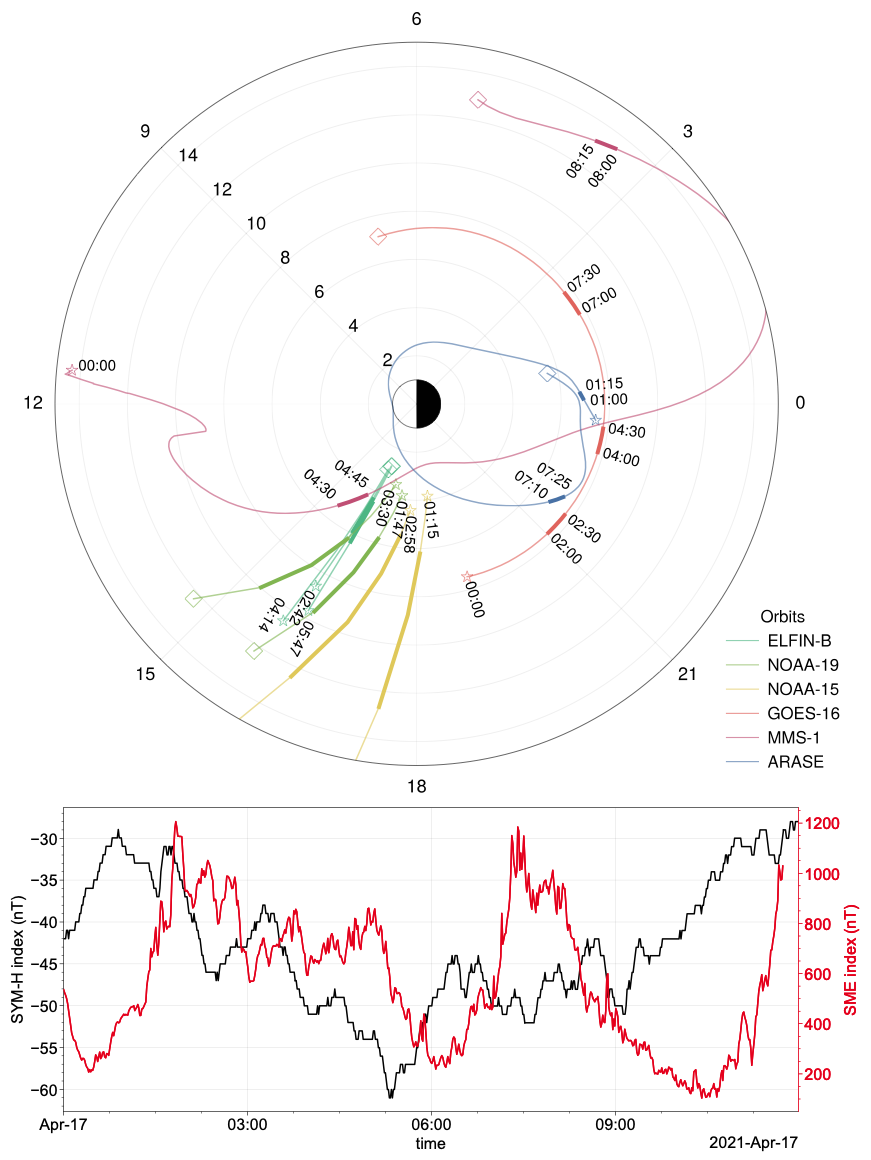
\includegraphics[width=0.6\textwidth,height=\textheight]{figures/fig1_orbit_multi_mission_conjunctions.png}

}

\caption{\label{fig-1}(top) An overview of the mission orbits recorded on April 17, 2021. The orbits of the various missions are projected onto the MLT and \(L\)-shell plane, using Tsyganenko model. (bottom) Sym-H and SME indices during this event.}

\end{figure}%

\begin{figure}

\centering{

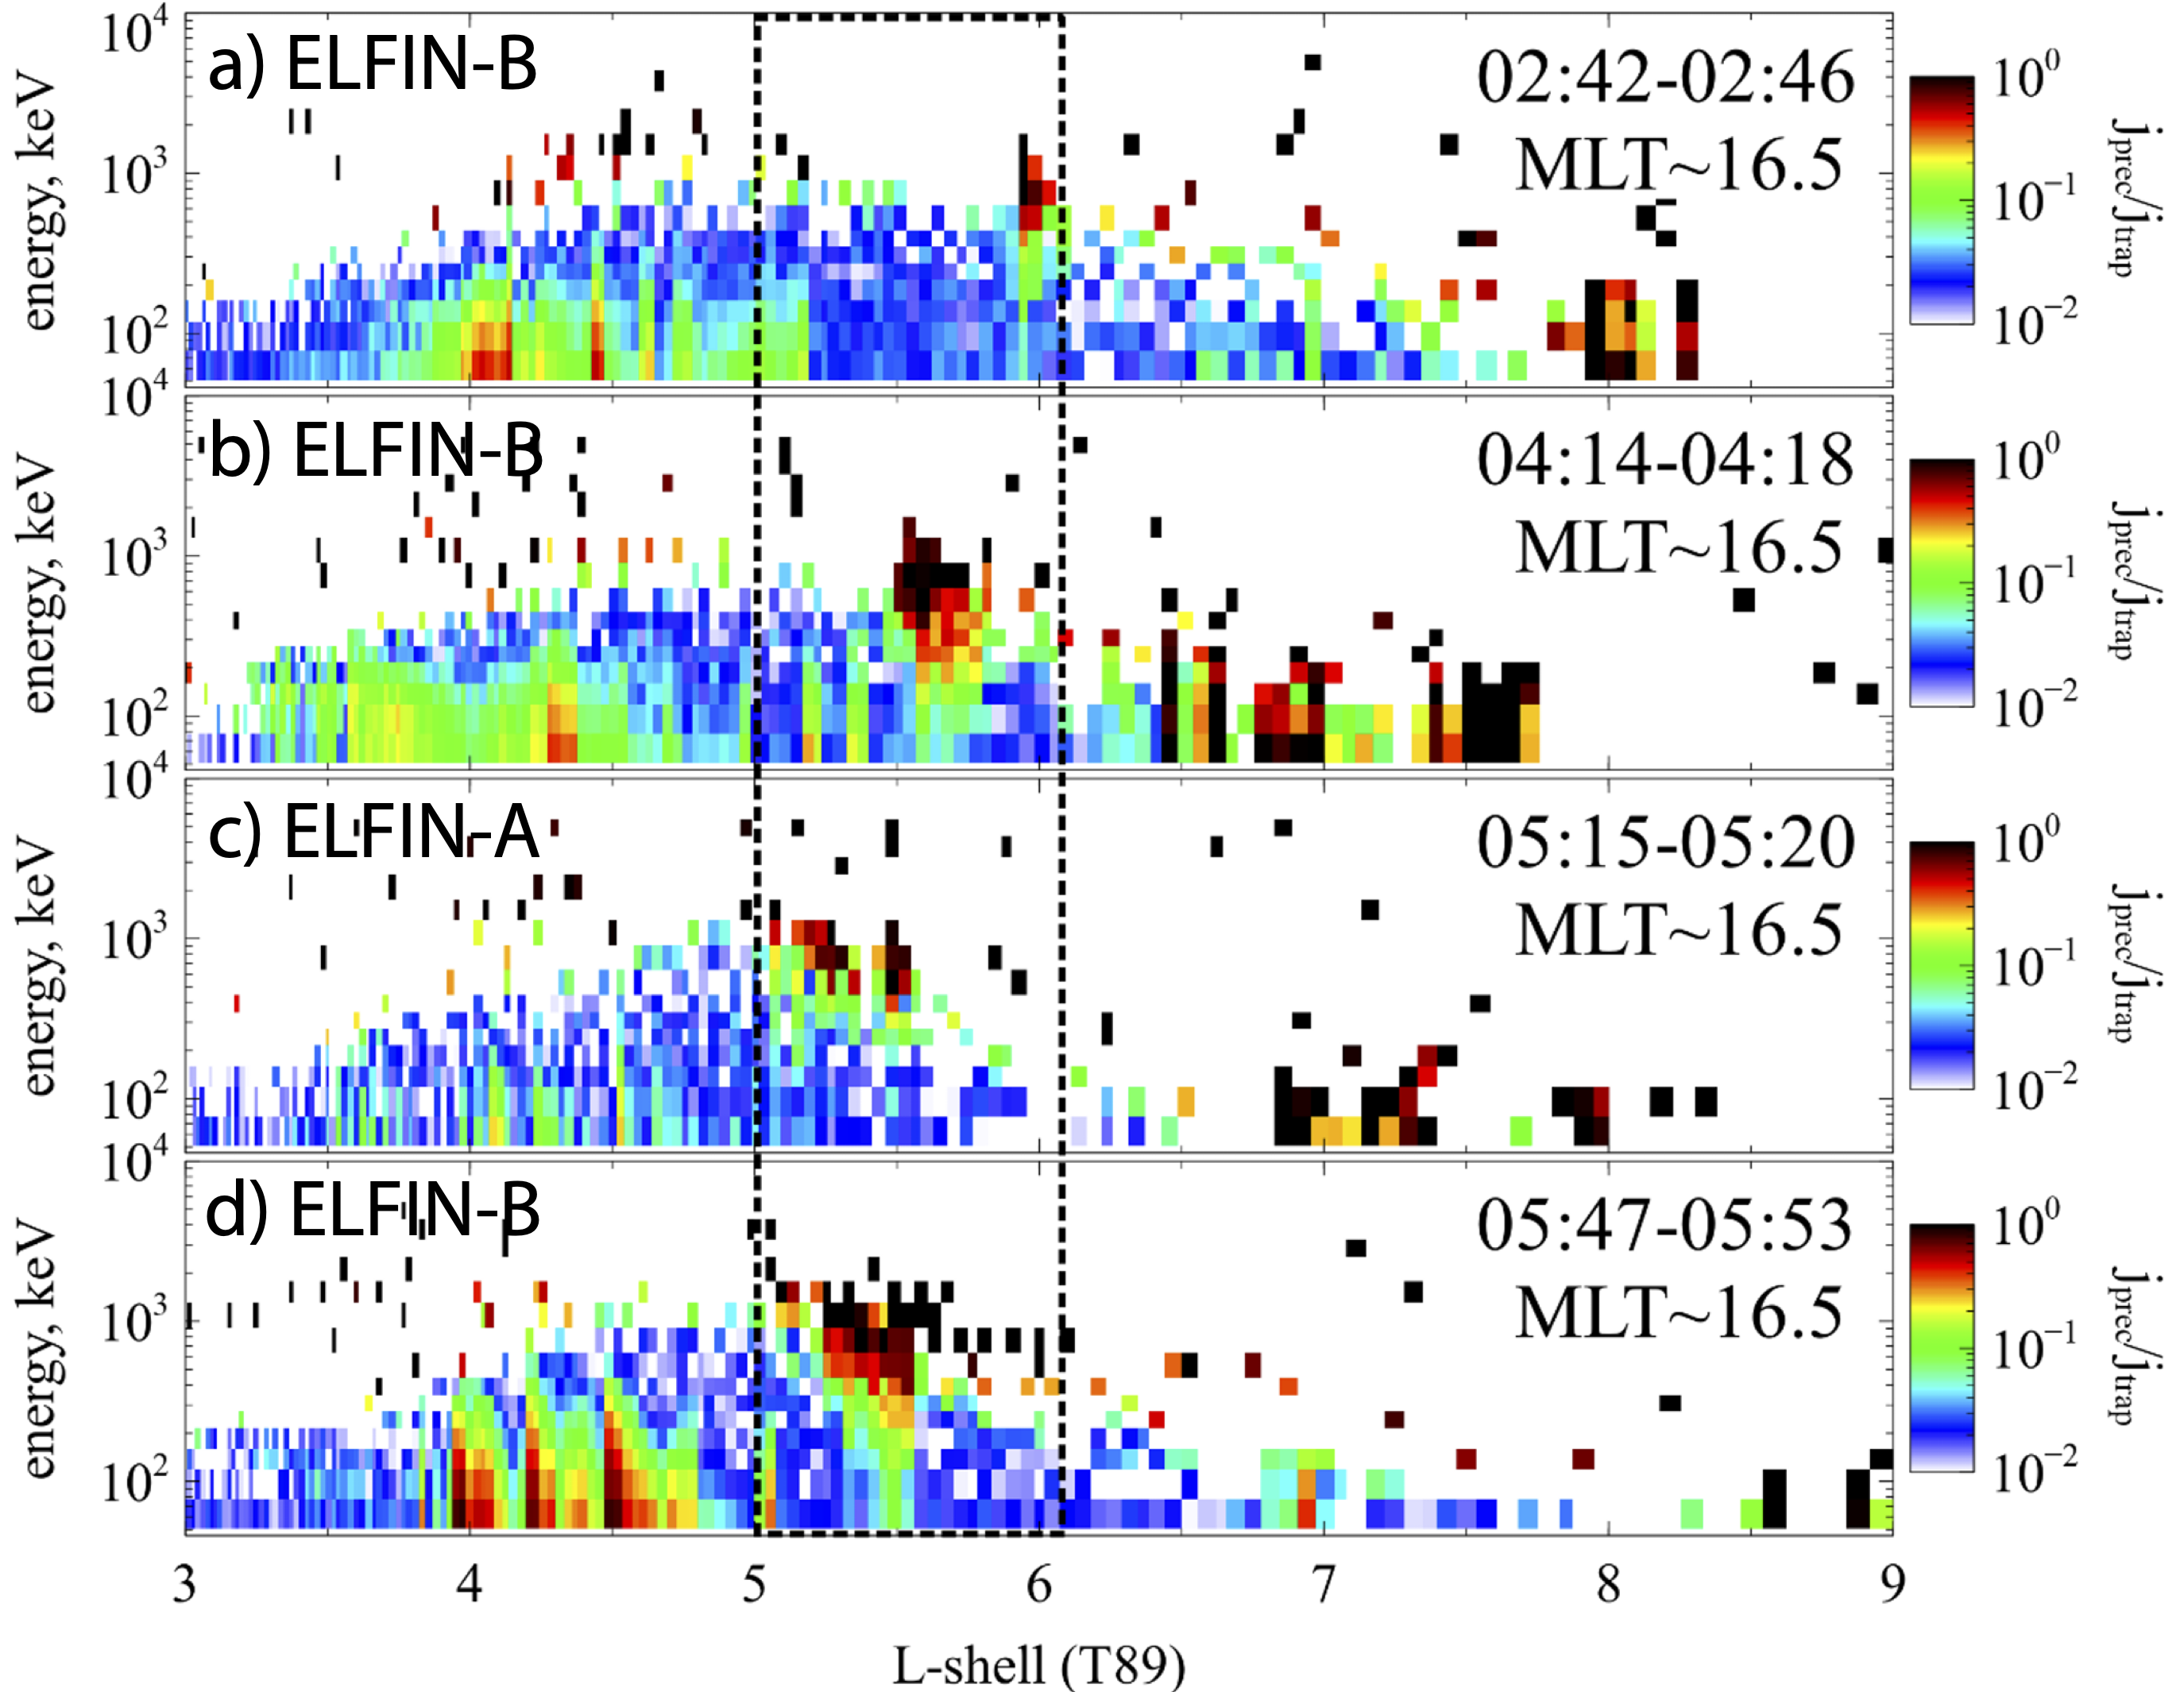
\includegraphics{figures/fig_elfin_j_ratio.png}

}

\caption{\label{fig-elfin}Two ELFIN CubeSats observations of EMIC wave-driven electron precipitation, where the precipitating flux reaches the trapped flux in high-energy channels, over an interval exceeding three hours, from 02:42 to 05:53 UT. The locations are projected to the equatorial L-Shell and MLT, using the Tsyganenko89 magnetic field model. Panels (a), (b), and (d) show data from ELFIN-B, while panel (c) features observations from ELFIN-A.}

\end{figure}%

\begin{figure}

\centering{

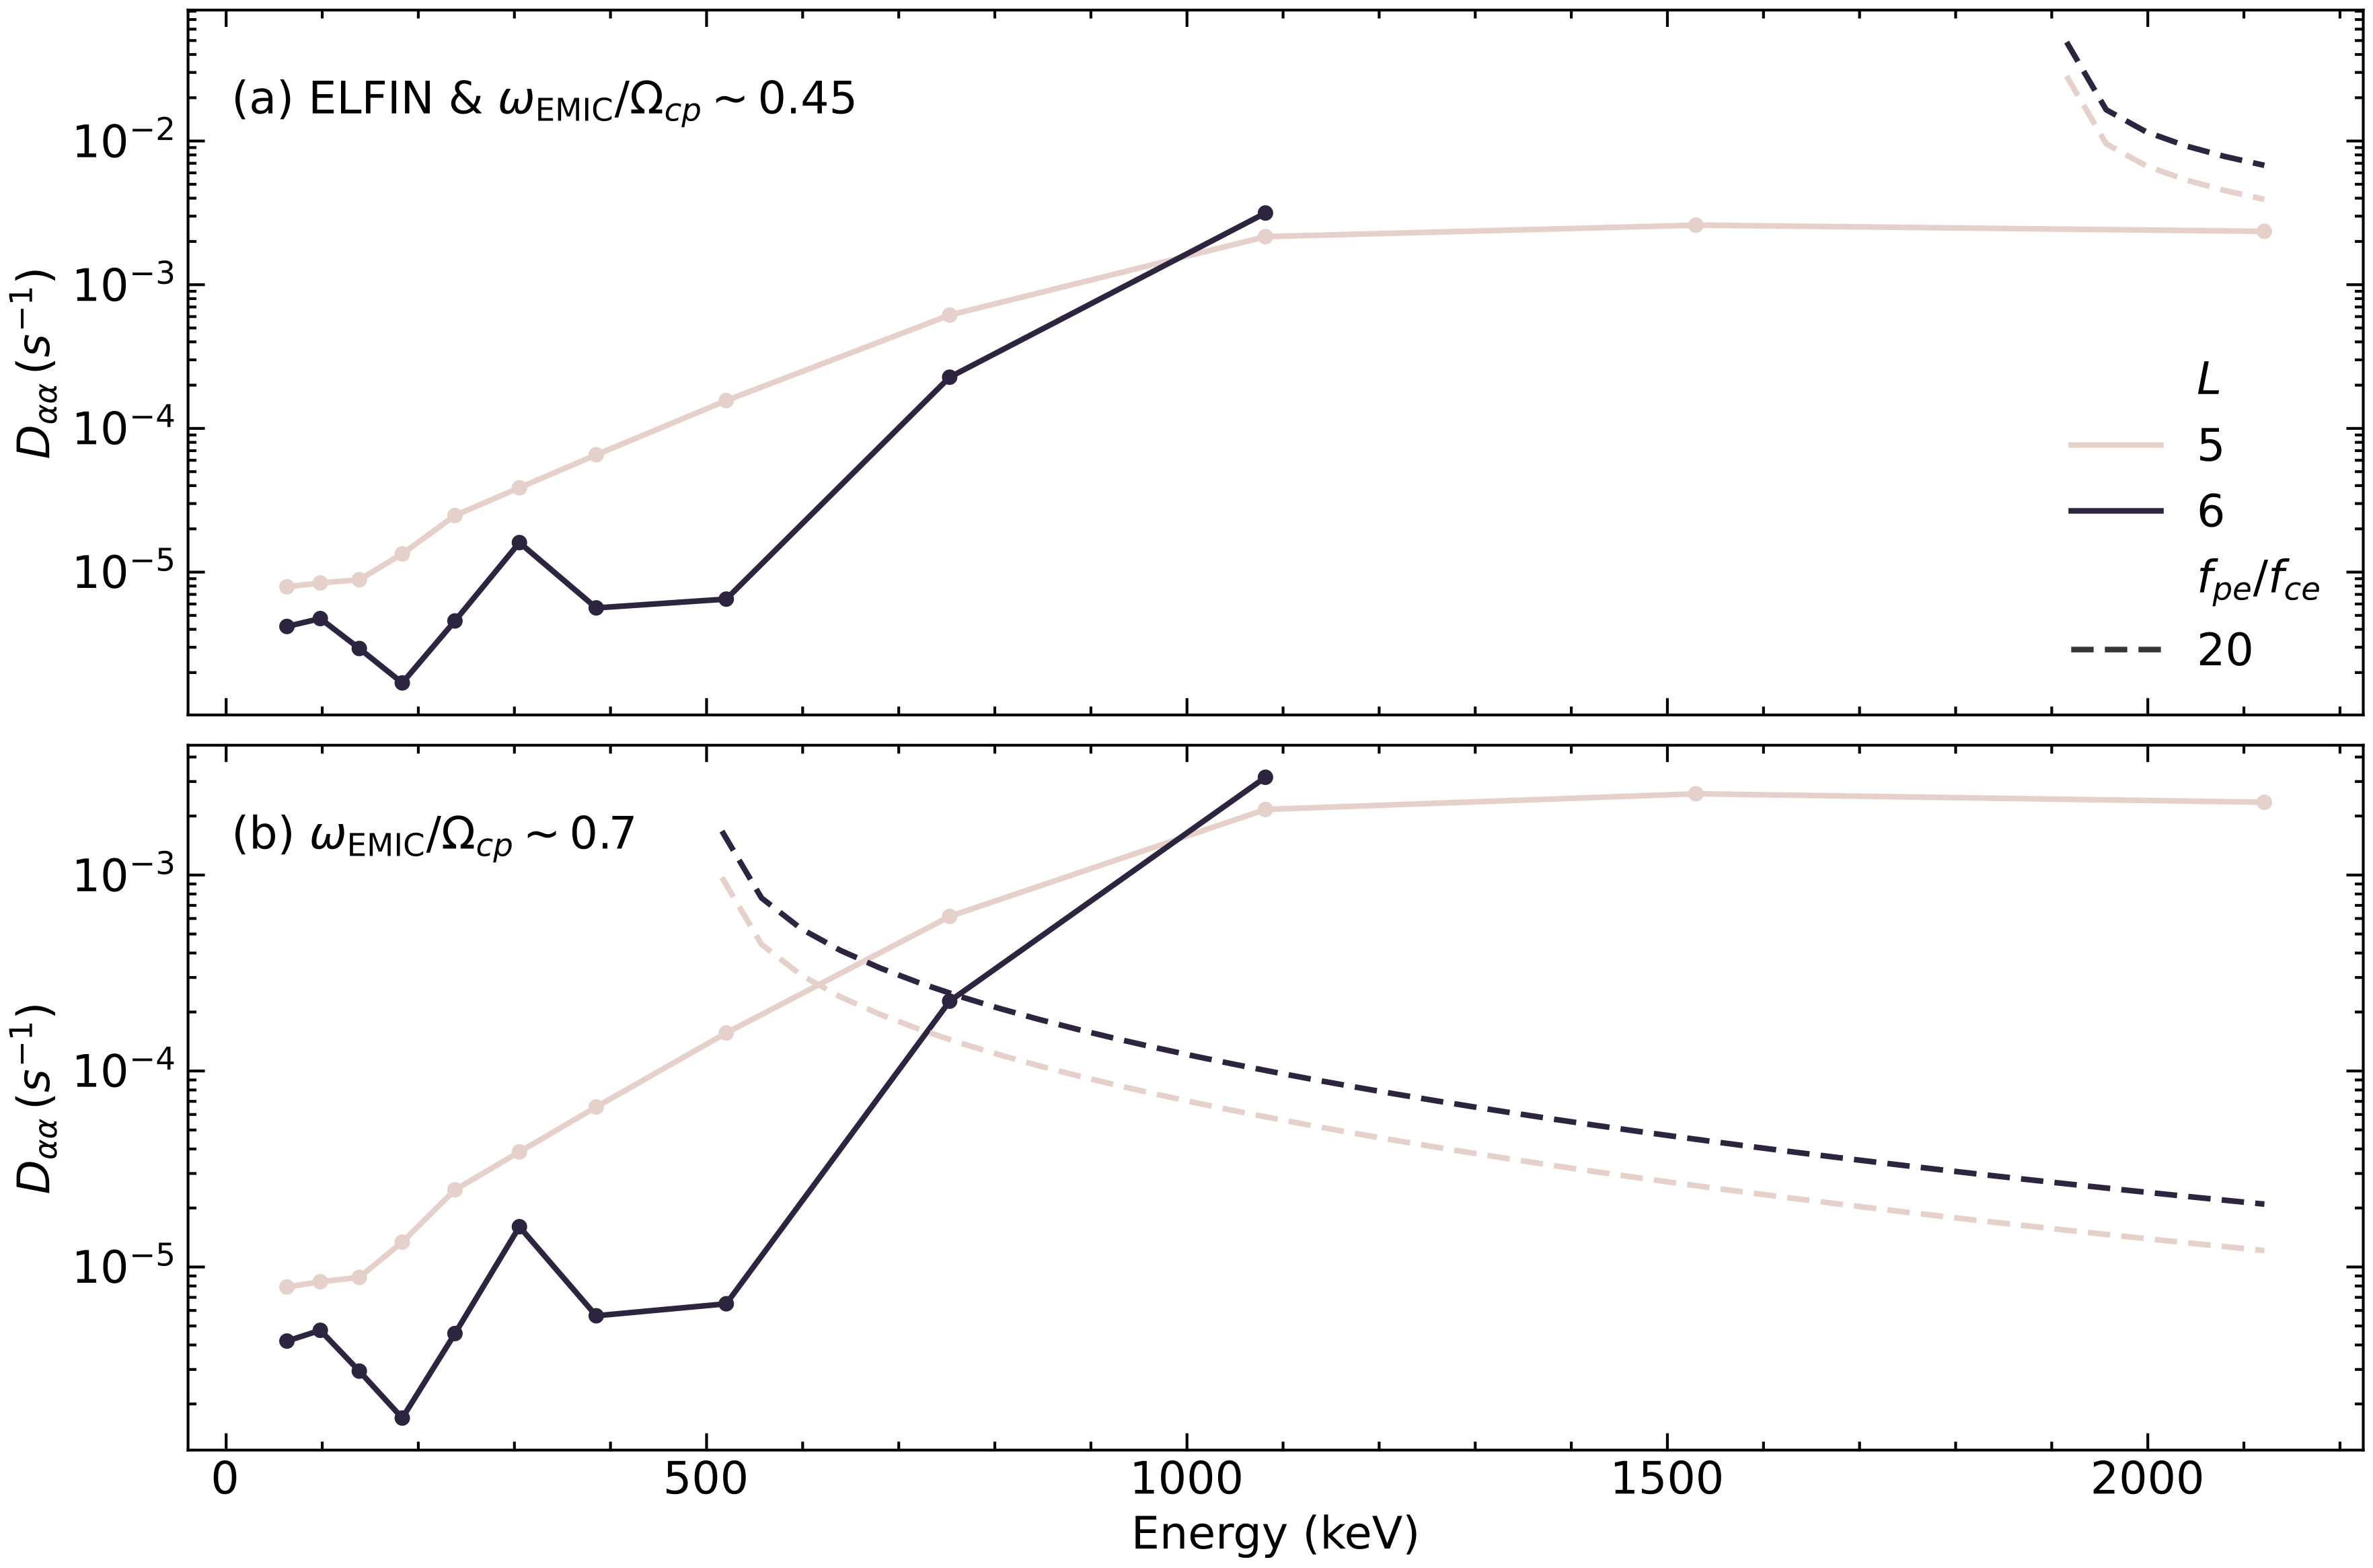
\includegraphics{figures/fig_Daa.png}

}

\caption{\label{fig-Daa_EMIC}Panel (a) Diffusion rates \(D_{\alpha\alpha}\) of electrons near the loss-cone inferred, using Equation 2, from ELFIN measurements of precipitating and trapped electron fluxes in the dusk sector near 16 MLT, at \(L=5\) (solid red) and \(L=6\) (solid black) as a function of electron energy \(E\). Diffusion rates \(D_{\alpha\alpha}\) near the loss-cone evaluated based on analytical estimates for H-band EMIC waves with typical wave and plasma parameters at \(L=5\) (red) and \(L=6\) (black) in a noon-dusk plasmaspheric plume, as a function of energy \(E\) are shown for a typical ratio \(f_{pe}/f_{ce}=20\), a peak wave amplitude of \(B_w=0.5\) nT at \(\omega_{\text{EMIC}}/\Omega_{cp}\sim 0.4\), and a (minimum) frequency \(\omega_{\text{EMIC}}/\Omega_{cp}\sim 0.45\) for cyclotron resonance with \(\sim2\) MeV electrons (dashed lines). (b) Same as (a) with analytical estimates of \(D_{\alpha\alpha}\) shown for H-band EMIC waves with a peak wave amplitude of \(B_w=0.5\) nT at \(\omega_{\text{EMIC}}/\Omega_{cp}\sim 0.4\) and a (minimum) frequency \(\omega_{\text{EMIC}}/\Omega_{cp}\sim 0.7\) for cyclotron resonance with \(\sim0.75\) MeV electrons (dashed lines).}

\end{figure}%

\newpage{}


  \bibliography{../../../../files/references.bib,../../../../../share/bibliography/research.bib}


\bibliography{files/Anton.addon.bib,files/Anton.full.bib,files/research.bib}

\end{document}
